\section{The Loop method}
Compact models are an efficient way to model the TSP with a polynomial number of
constraints. However, they allow solving only small instances since they still
have a huge number of them. A more efficient way to avoid subtours would be to
generate the subtour elimination constraints on the fly, only when needed while
precisely targeting a subtour elimination.\\
Benders method is a general strategy to solve MIP problems: it starts solving a
reduced version of the model (in which some constraints, even those that ensures
correctness, are relaxed) and then it adds to the model that constraints that
would be violated (according to actual solution) if present from the beginning.
Then it repeats the procedure until a correct solution is obtained.\\
Applied to TSP: we start from an SEC-free model that will produce subtours, we
solve it using a MIP solver as a black box until we found a solution with
subtours. For each of them, we have to add to the model Danzing's SEC: this will
prevent those subtour to form the next iteration. We repeat this until a
single-tour solution is obtained.

\begin{algorithm}[H]
\SetAlgoLined
\KwResult{A subtour-free solution}
    \emph{model} $\leftarrow$ prepare SEC-free model\;
    \emph{sol} $\leftarrow$ MIP opt (\emph{model})\;
    \While{sol contains subtours}{
        \ForEach{subtour s in sol} {
            add to \emph{model} Danzing's SEC that involves $s$
        }
        \emph{sol} $\leftarrow$ MIP opt (\emph{model})
    }
    \caption{The Loop method}
\end{algorithm}

Since it uses a MIP solver as a black box inside a loop, we will refer to it as
the \emph{Loop method} or, improperly since it is its generalization,
\emph{Benders method}.

There's no reason to use an asymmetric version of the problem, the symmetric one will works well. Danzing's SEC
that will be added at each iteration became:

\begin{equation*} 
    \begin{array}{rrlr} 
        \displaystyle\sum_{i,j \in S,\ i \neq j} x_{ij} & \le |S|-1 & \forall S \subset V: |S| \ge 3
    \end{array} 
\end{equation*}

Notice that the number of non-zero on the left-hand side of the constraint is
${|S|\choose 2} \in \mathcal{O}(|S|^2)$ and that we are considering subset $S$
of at least dimension 3: for dimension 2 the constraint is clearly absorbed in
the variable's bounds ($x_{ij} \le 1$).

\begin{figure}[h]
    \centering
    \begin{minipage}{.45\textwidth}
        \centering
        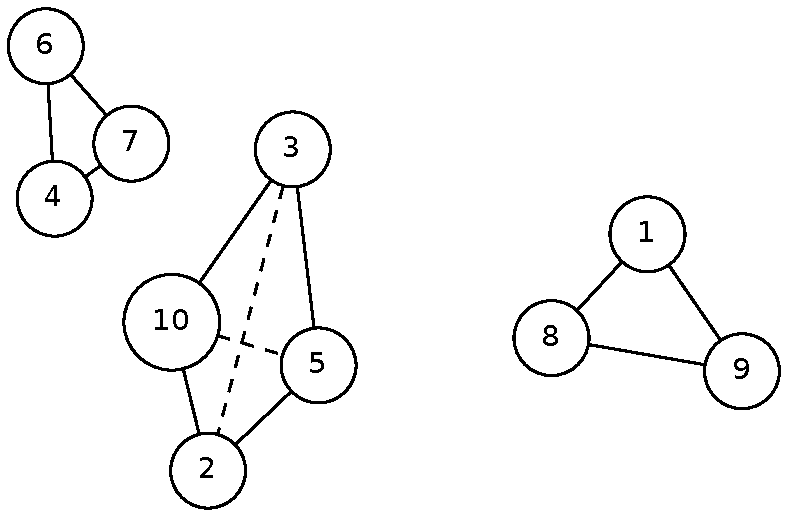
\includegraphics[width=0.8\linewidth]{figures/bendersa}
        \label{fig:sub1}
    \end{minipage}%
    \begin{minipage}{.1\textwidth}
        $\implies$
    \end{minipage}%
    \begin{minipage}{.45\textwidth}
        \centering
        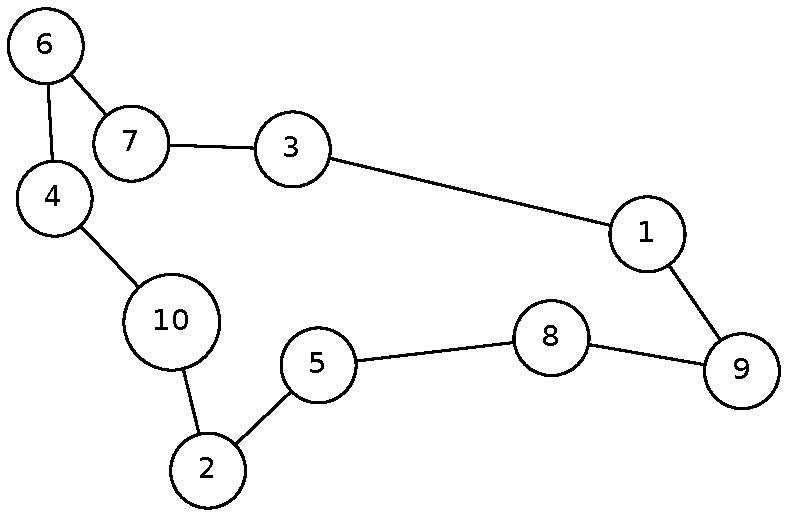
\includegraphics[width=0.8\linewidth]{figures/bendersb}
        \label{fig:sub2}
    \end{minipage}
    \caption[Benders example]{\centering Adding $x_{47} + x_{76} + x_{64} \le 2$, $x_{25} + x_{53} +
    x_{310} + x_{102} + x_{23} + x_{510} \le 3$ and $x_{89} + x_{91} + x_{18} \le
    2$ will prevent subtours to form, forcing a subtour-free solution}
\end{figure}

One thing that's important to keep in mind is that, during iterations, there's
no guarantee that the number of subtours is monotone nor decreasing. After some
iterations, let's say when such number are less than 5, we can have lots of
variability and the convergence to a single tour can be pretty slow. Also,
there's no thing such as subtours merging: adding two SEC doesn't mean that
those subtours will be merged in a single one, they can also form subtours in
other ways.

\subsection{Implementation details}
The last thing to specify are some details left behind. The MIP solver
that we will use is CPLEX. We can have more freedom in the connected component
algorithm, necessary for the creation of the constraints. We need both fast
insertion and fast retrieve the nodes of a component. This can be done adapting
a union-find data structure (with path compression and other heuristics) mixed
with a linked-list (implemented using swap ends trick). Notice that it's not
necessary to preserve the order of the subtour visit, we only need the nodes
that belongs to the same component. This could have been the best idea if the
number of subtours would be monotonically decreasing. Anyway, that idea works,
but it's a huge overkill, a simple successor vector (by sacrificing retrieve
time) or an adjacency list (specialized keeping 2 slots for node) can do the job
flawlessly. The second option is actual implemented, because it is reused in
future approaches to TSP. We have to state that the most of time will be spent
by the MIP solver, that will occupy the majority of the  available time limit.

\section{The Two-phase Loop method}
The time limit management for the Loop method is trivial: the MIP solver, for
the current iteration, can take advantage of the remaining time limit, that
will be split during each iteration. But, it's possible to notice, that after
some iteration the model became bigger and bigger (because of the SEC added)
and the MIP solver uses more and more time to solve the problem the single
subproblem. For this reason, considering an initial phase (phase 1) when we're
not interested in optimality, we can set a lower and fixed time limit for those
iterations, and so generate useful SEC to solve the problem. At the end of this
phase, even if we reach a single-tour solution, we cannot claim its optimality,
because we fixed our MIP solver to run constrained in time. We have then to let
run the solver indefinitely to reach an optimal solution (phase 2), as we did in
the usual Loop method. 

Since managing the time limit of CPLEX is too platform-dependent it's
possible to fix the maximum number of nodes generated or the maximum number of
incumbent updates: both of them behave like a time limit for phase 1's
iterations. The first strategy (setting \texttt{CPX\_PARAM\_NODELIM} in CPLEX)
is implemented.

We will refer this strategy as \emph{Two-phase Loop method}.

\begin{claim} 
    The improvement given by Two-phase Loop method is negligible.
\end{claim}

\begin{figure}[h]
    \centering
    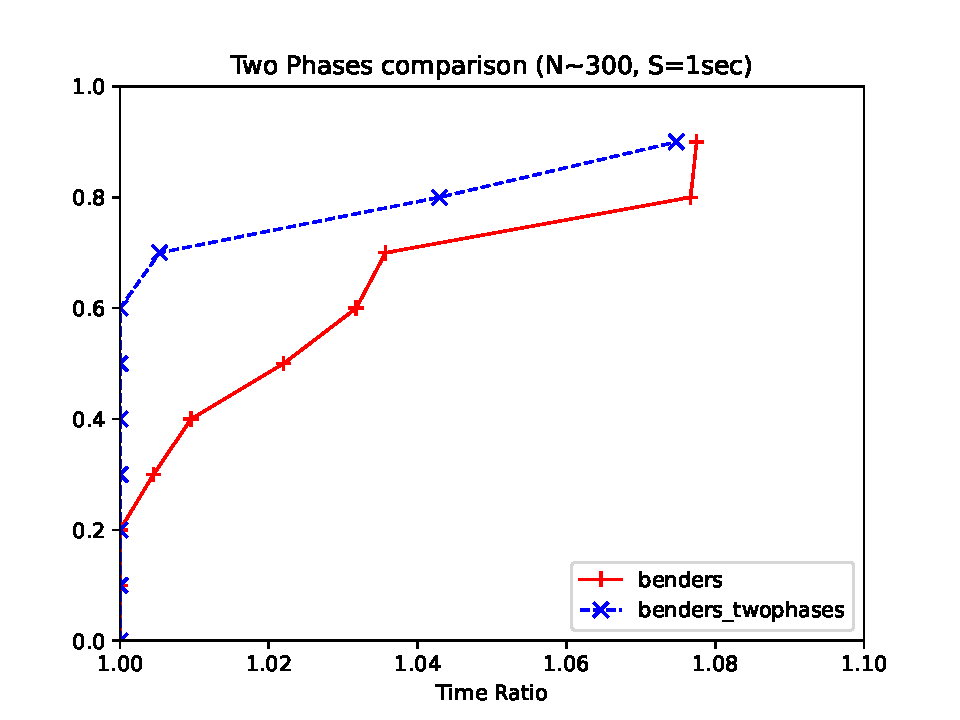
\includegraphics[width=0.8\textwidth]{figures/benders2phases}
    \caption{Loop methods comparison, short time ratio}
\end{figure}

Two hyperparameters have to be fixed, the amount of time spent on phase 1 and
the maximum number of branching nodes. We are not going to perfectly tune those
parameters, because performance variability will destroy our analysis, so,
after some tests on a validation set trying different parameters, we will fix
those to reasonable values: phase 1 will take 50\% of the time available,
during which only 3 nodes will be processed. More important details on
parameters tuning in appendix \ref{appendix:tuning}\\ The difference is
negligible, considering the very short time ratio, the two methods can be
considered equally valid.\\ Another reasonable strategy is to leave phase 2 the
shortest amount of time to solve to optimum the problem while using the
remaining time on phase 1. This strategy is better than the pure Loop method,
but the fifty-fifty split of time between phases seems the best.

\section{Callbacks method}
An adaptation of Benders method can be achieved using CPLEX's features:
\emph{callbacks}, a simple way to inject user-written code during
branch-and-cut. CPLEX uses branch-and-cut to solve MIP problems and, for each
node (excluding the special case of root node where some preprocessing also
happens), the fractional result obtained from LP relaxation is cut also using
cut pool's cuts to obtain an integer solution, then some primal
heuristics are applied to obtain a solution which will helpfully update the
incumbent. During these two phases (cuts application and before the incumbent
update) it's possible to generate and add constraints to the model using the
mechanism of callbacks. The idea behind this approach is that the user has more
insight than CPLEX about the problem, so it can add more specific and
problem-related cuts that will improve the computation.

This is different from Benders method, but the idea is similar: start
with SEC-free model, then adds, taking advantage of callbacks, all the SEC
necessary until a single-tour solution is obtained. We will refer to this method
as the \emph{Benders Callbacks method}.

The SEC added are, again, Danzing's SEC for symmetric version, but in two
different fashion. When adding a SEC before the incumbent update, it's possible to
recycle the connected components algorithm because an integer solution is
provided. The situation is different when trying to generate a SEC in the cut
callback because the code will be called back just after LP relaxation
solution, so just a fractional solution is available, and such a solution is a
mess, because we have some edges that are fixed to one and some other not, so
clearly not a collection of cycles. Anyway, an algorithm for finding connected
components given a fractional solution exists, and it relies on solving a
series of max-flow problems. Since the implementation is troubling, it's
possible to exploit a well-known library that will provide a subtour separation
procedure: \emph{Concorde}. The library's function for that task will be called
during the cut callback and some SEC will be added to the model. Those
constraints, as opposed to those generated before updating the incumbent, are
\emph{user
cuts}\footnote{\href{https://www.ibm.com/docs/en/cofz/12.8.0?topic=pools-what-are-user-cuts-lazy-constraints}{https://www.ibm.com/docs/en/cofz/12.8.0?topic=pools-what-are-user-cuts-lazy-constraints}}:
they are not needed to generate a feasible solution (single-tour) since we
already add all the useful SEC before the incumbent update, but they will help to
tight the model.

Let's now focus on the user cuts generation procedure. Considering the number of
nodes generated during branch-and-cut, the possible huge amount of SEC that are
possible to generate, the computing time required to generate those SEC, and the
fact that we're making our model bigger, one may ask if there this procedure
will add some overhead to CPLEX computation. The answer is positive: a model
with lots of SEC is great because it will tight the formulation, but considering
the amount of time spent generating those constraints and spent during
relaxations, it's necessary to find a trade-off. Some possible strategies are to
stop the generation of constraints if some requirements are reached. We're going
to present two strategies, by avoiding the separation randomly (per node) or
after a fixed number of nodes.
\newpage

\begin{claim}
    The Benders idea implemented through callbacks is superior to the Loop
    method. Stopping the constraint generation after a fixed number of nodes seems
    a good trade-off.
\end{claim}

\begin{figure}[h]
    \centering
    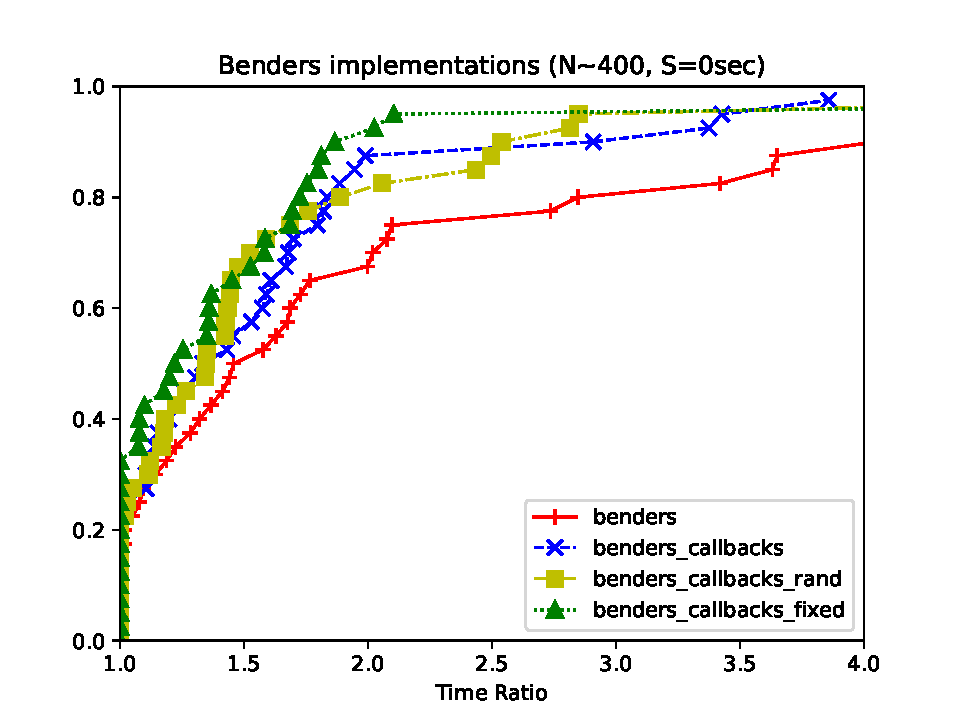
\includegraphics[width=0.8\textwidth]{figures/benders_final}
    \caption{Benders implementation comparison, with variants in callbacks}
\end{figure}

The comparison is done considering 40 instances of around 400 nodes each. Four
models have been compared: the Loop method and three variant of the callbacks
method: in one of them we stop the SEC generation (after LP relaxation) per node
randomly with 50\% probability, in another one, we stop after 64 nodes, and in
the third one we didn't stop the process at all, by adding as many constraints
as possible.\\
The hyperparameters we considered, 50\% and 64 nodes, are tuned using a
validation test, but not tuned to perfection considering performance
variability. Anyway, they both seem reasonable. Considering that with 400 nodes
per instance, the branching tree has usually $>10k$ nodes. The 50\% random
strategy simply cut by half all the possible SEC to be added. The fixed node
strategy is more like a bet: 64 nodes are way less than the total number of node
in the branching tree, we bet that the first explored nodes contain useful SEC to
be separated. 64 is chosen to be the first 5 levels in the branching tree,
considering a \emph{go-wide} strategy decided by CPLEX or the first 64 if CPLEX
decided to \emph{go-deep}. In this last case, we even bet on CPLEX's decision
ability.\\

The results show that the Loop method is inferior compared to the callbacks
method. The fixed nodes strategy seems slightly better than the other two, even
if the random strategy becomes competitive for a small slice of the time ratio. 
Anyway, both of them seem reasonable.
